\section{Background}
\label{sec-bg}
In this section, we briefly discuss the relevant background on BPFS \cite{c10}, a file system for byte addressable persistent memory. BPFS is one of the earliest file systems to be proposed for non-volatile memory systems and the authors showed that simply running a disk-based traditional file system on top of persistent memory is not enough to provide high performance. We first introduce the BPFS file system layout and discuss why the design is limited in terms of the cost of storage and volume of storage. We also briefly describe the techniques proposed in BPFS to achieve consistency and how they achieve atomicity and write ordering. We then describe the changes made to the persistent data structures and file system code to support a disk backed secondary storage in a subsequent section.

\subsection{BPFS Layout}
BPFS stores all the file system meta data and data in the form of a tree structure consisting of fixed-size blocks of 4KB in the non-volatile memory. Figure~\ref{fig-bpfstree} depicts the file system organization in BPFS. The BPFS file system consists of three kinds of files namely inode file, directory file and data file with each of these in turn arranged as a tree. The inode file is represented by a tree structure with the root of the inode file serving as the root of the file system. The location of this root node is stored at a known location in the non-volatile memory. Each of the leaves in the inode file contains an array of inode structures with each inode structure representing either a file or a directory. This inode structure contains the pointer to the root of the file or directory that the inode represents. The leaves of a data file tree are the data blocks and the leaves of a directory file tree are the directory entries.

\begin{figure}
\centering
\vspace{-0.2in}
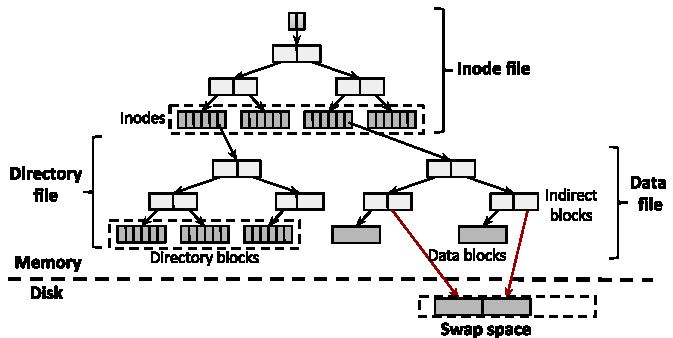
\includegraphics[width=0.5\textwidth]{figs/bpfs2.pdf}
\vspace{-0.2in}
\mycaption{fig-bpfstree}{BPFS tree structure}{\footnotesize The figure shows the file system organization of BPFS, along with our proposed modifications.}
\end{figure}

\subsection{File System Consistency}
BPFS maintains file system consistency employing a technique called short-circuit shadow paging. Shadow paging is a copy on write technique, where to modify a node in the tree a copy is made and the data is written to the copy. This requires updates of indirect pointers, which in turn triggers copy on writes on these indirect pointer blocks and this bubbles up to the root of the file system. Short-circuit shadow paging is an optimization, where the byte-addressability and atomic 64-byte write guarantee provided by NVM, makes in-place updates feasible. Hence, in-place updates are performed whenever possible. Short-circuit shadow paging guarantees that file system operations will commit atomically and in program order. Ordering is provided by hardware primitive called epoch barriers. In a disk based file system, for the writes to be durable, we need to flush the operating system buffer cache. Similarly, for the data to be durable in NVM, we have to flush the CPU caches. BPFS provides the guarantee that data is made durable as soon on \textit{fsync} operation by flushing the CPU caches.
